\begingroup
\fenicschapter{Automated testing of saddle point stability conditions}
              {Automated testing of saddle point stability \\ conditions}
              {Automated testing of saddle point stability conditions}
              {Marie E. Rognes}
              {rognes}

\newcommand{\rognesc}{c}
\newcommand{\rognestriang}{\mathcal{T}}

\newcommand{\rognesvectorcg}[2]{[\mathrm{CG}_{#1}]^{#2}}
\newcommand{\rognescg}[1]{\mathrm{CG}_{#1}}
\newcommand{\rognesrt}[1]{\mathrm{RT}_{#1}}
\newcommand{\rognesdg}[1]{\mathrm{DG}_{#1}}
\newcommand{\rognesascot}{ASCoT}
\newcommand{\rognespython}{Python}

\index{mixed finite element method}
\index{discrete stability}

Over the last five decades, there has been a substantial body of
research on the theory of mixed finite element methods.  Mixed finite
element methods are finite element methods where two or more finite
element spaces are used to approximate separate variables.  These
methods have often been applied to saddle point problems arising from
constrained minimization problems. Examples include the Stokes
equations, the equations of Darcy flow (or the mixed Laplacian) or the
Hellinger--Reissner formulation for linear elasticity.  For equations
involving several variables, and where elimination of any of the
variables is not a viable option, the usefulness of such methods is
evident. For other equations, discretizations based on the
introduction of additional variables may have improved properties.
The goal of this chapter is to demonstrate that one may automate the
examination of the stability of any given discretization.

\section{Background}

For any discretization of a variational problem, stability is crucial
to ensure well-posedness. For coercive problems, the discrete
stability may often be easily ensured. For mixed discretizations of
saddle point problems on the other hand, stability may be a nontrivial
affair. Indeed, the mixed finite element spaces must usually be
carefully chosen. The stability theory for mixed finite element
discretizations originates from the work of \citet{Babuvska1972/73}
and \citet{Brezzi1974} in the early 1970's. Brezzi established two
conditions ensuring the stability of a mixed finite element
discretization of a canonical saddle point problem.  Since then, many
papers (and books) have been devoted to the identification and
construction of specific stable mixed finite elements for specific
saddle point problems~\citep{ArnoldFalkWinther2006,
BrezziDouglasMarini1985, BrezziFalk1991, BrezziFortin1991,
RaviartThomas1977, TaylorHood1973}. Some of the analytical results are
well known, such as the stability of the Taylor--Hood elements for the
Stokes equations~\citep{BrezziFalk1991, Stenberg1984, TaylorHood1973}.
Others, such as the reduced stability of the
$\rognesvectorcg{1}{2} \times
\rognesdg{0}$ elements on criss-cross triangulations for the mixed
Laplacian~\citep{BoffiBrezziGastaldi2000}, may be less so.

As stated above, the goal of this chapter is to demonstrate that the
process of numerically examining the stability of any given
discretization can be automated.  For a given discretization, the
Brezzi constants are computable through a set of eigenvalue
problems. These eigenvalue problems have previously been used to
numerically study the stability of certain
discretizations~\citep{ArnoldRognes2009, ChapelleBathe1993,
Qin1994}. However, automation of this task has not been previously
considered in the literature. A secondary aim is to show that the
automation process is fairly easy given a software framework
supporting the following components: a suitable range of different
finite element spaces, easy support of bilinear forms defining
equations and inner products, and finally, a linear algebra backend
with support for generalized, possibly singular, eigenvalue
problems. The components of the \fenics{} project provide these tools.

An automated stability tester provides several advantages. First, the
notion of saddle point stability goes from something rather abstract
to something rather hands-on. Moreover, even a novice user can easily
get an overview of the available stable (or unstable) finite elements
for a given equation. For research purposes, it provides a tool for
the careful examination of discretizations that have stability
properties depending on the tessellation structure. In particular,
this framework has been used to study the stability properties of
Lagrange elements for the mixed Laplacian~\citep{ArnoldRognes2009}.

This chapter is organized as follows. For motivational purposes, a
simple example illustrating the importance of discrete stability is
presented in Section~\ref{rognes:sec:motivation}. The subsequent two
sections summarize the discrete stability theory of \babuska{} and
Brezzi and how the stability constants involved can be computed
through a set of eigenvalue problems. In
Section~\ref{rognes:sec:automation}, a strategy for the automation of
numerical stability testing is presented. In particular, a
light-weight \rognespython{} module, \rognesascot{}~\citep{Rognes2009},
constructed on top of DOLFIN~\citep{LoggWells2010}, is described. This
module is freely available as a \fenics{} Application
at \url{https://launchpad.net/ascot}. The use and capabilities of this
framework are demonstrated when applied to two classical examples: the
mixed Laplacian and the Stokes equations in
Section~\ref{rognes:sec:examples}. Finally,
Section~\ref{rognes:sec:conclusion} provides some concluding remarks
and a discussion of limitations.

\section{Why does discrete stability matter?}
\label{rognes:sec:motivation}

\looseness-1{}The following simple example illustrates that discrete stability is
indeed crucial for the approximation of saddle point problems. Let
$\Omega = (0, 1)^2$ be the unit square in $\R^2$, and take $f = - 2
\pi^2 \sin(\pi x) \sin(\pi y)$. Consider the following mixed
formulation of the Poisson problem with homogeneous Dirichlet boundary
conditions: for the given data $f \in L^2(\Omega)$, find $\sigma \in
H(\Div, \Omega)$, and $u \in L^2(\Omega)$ such that
\begin{equation}
  \label{rognes:eq:mixedlaplace}
  \begin{split}
    \langle \sigma, \tau \rangle + \langle \Div \tau, u \rangle &= 0
    \quad\quad \foralls \tau \in H(\Div, \Omega), \\
    \langle \Div \sigma, v \rangle &= \langle f, v \rangle
    \quad \foralls v \in L^2(\Omega).
  \end{split}
\end{equation}
This problem is well-posed: such solutions exist, are unique and
depend continuously on the given data. In particular, $u = \sin(\pi x)
\sin(\pi y)$ and $\sigma = \Grad u$
solve~\eqref{rognes:eq:mixedlaplace}.

Next, let $\rognestriang_h$ be a uniform triangulation of the unit
square that is formed by dividing the domain into $n \times n$
subsquares (with $h$ the maximal triangle diameter) and dividing each
square by the diagonal with positive slope. Given a pair of finite
element spaces $\Sigma_h \times V_h$ defined relative to this
tessellation, the equations~\eqref{rognes:eq:mixedlaplace} can be
discretized in the standard manner: find $\sigma_h \in \Sigma_h$ and
$u_h \in V_h$ such that
\begin{equation}
  \label{rognes:eq:mixedlaplace:discrete}
  \begin{split}
    \langle \sigma_h, \tau \rangle + \langle \Div \tau, u_h \rangle &= 0
    \quad\quad \foralls \tau \in \Sigma_h, \\
    \langle \Div \sigma_h, v \rangle &= \langle f, v \rangle
    \quad \foralls v \in V_h.
  \end{split}
\end{equation}
The final question becomes what finite element spaces $\Sigma_h$ and
$V_h$ to choose. As we shall see, the well-posedness of the discrete
problem will heavily rely on the choice of spaces.

First, let us consider a naive choice; namely, taking the space of
continuous piecewise linear vector fields defined relative to
$\rognestriang_h$ for the space $\Sigma_h$ and the space of continuous
piecewise linears for $V_h$. This choice turns out to be a rather bad
one: the finite element matrix associated with this pair will be
singular! Hence, there does not exist a discrete solution $(\sigma_h,
u_h)$ with this choice of $\Sigma_h \times V_h$.

As a second attempt, we keep the space of continuous piecewise linear
vector fields for $\Sigma_h$, but replace the previous space $V_h$ by
the space of piecewise constant functions. This pair might appear to
be a more attractive alternative: there does indeed exist a discrete
solution $(\sigma_h, u_h)$. However, the discrete solution is not at
all satisfactory. In particular, the approximation of the scalar
variable $u_h$ is highly oscillatory,
see~Figure~\ref{rognes:fig:example}\subref{rognes:fig:cg}, and hence
it is a poor approximation to the correct solution.
%%\begin{figure}
%%  \centering
%%  {\label{rognes:fig:cg} 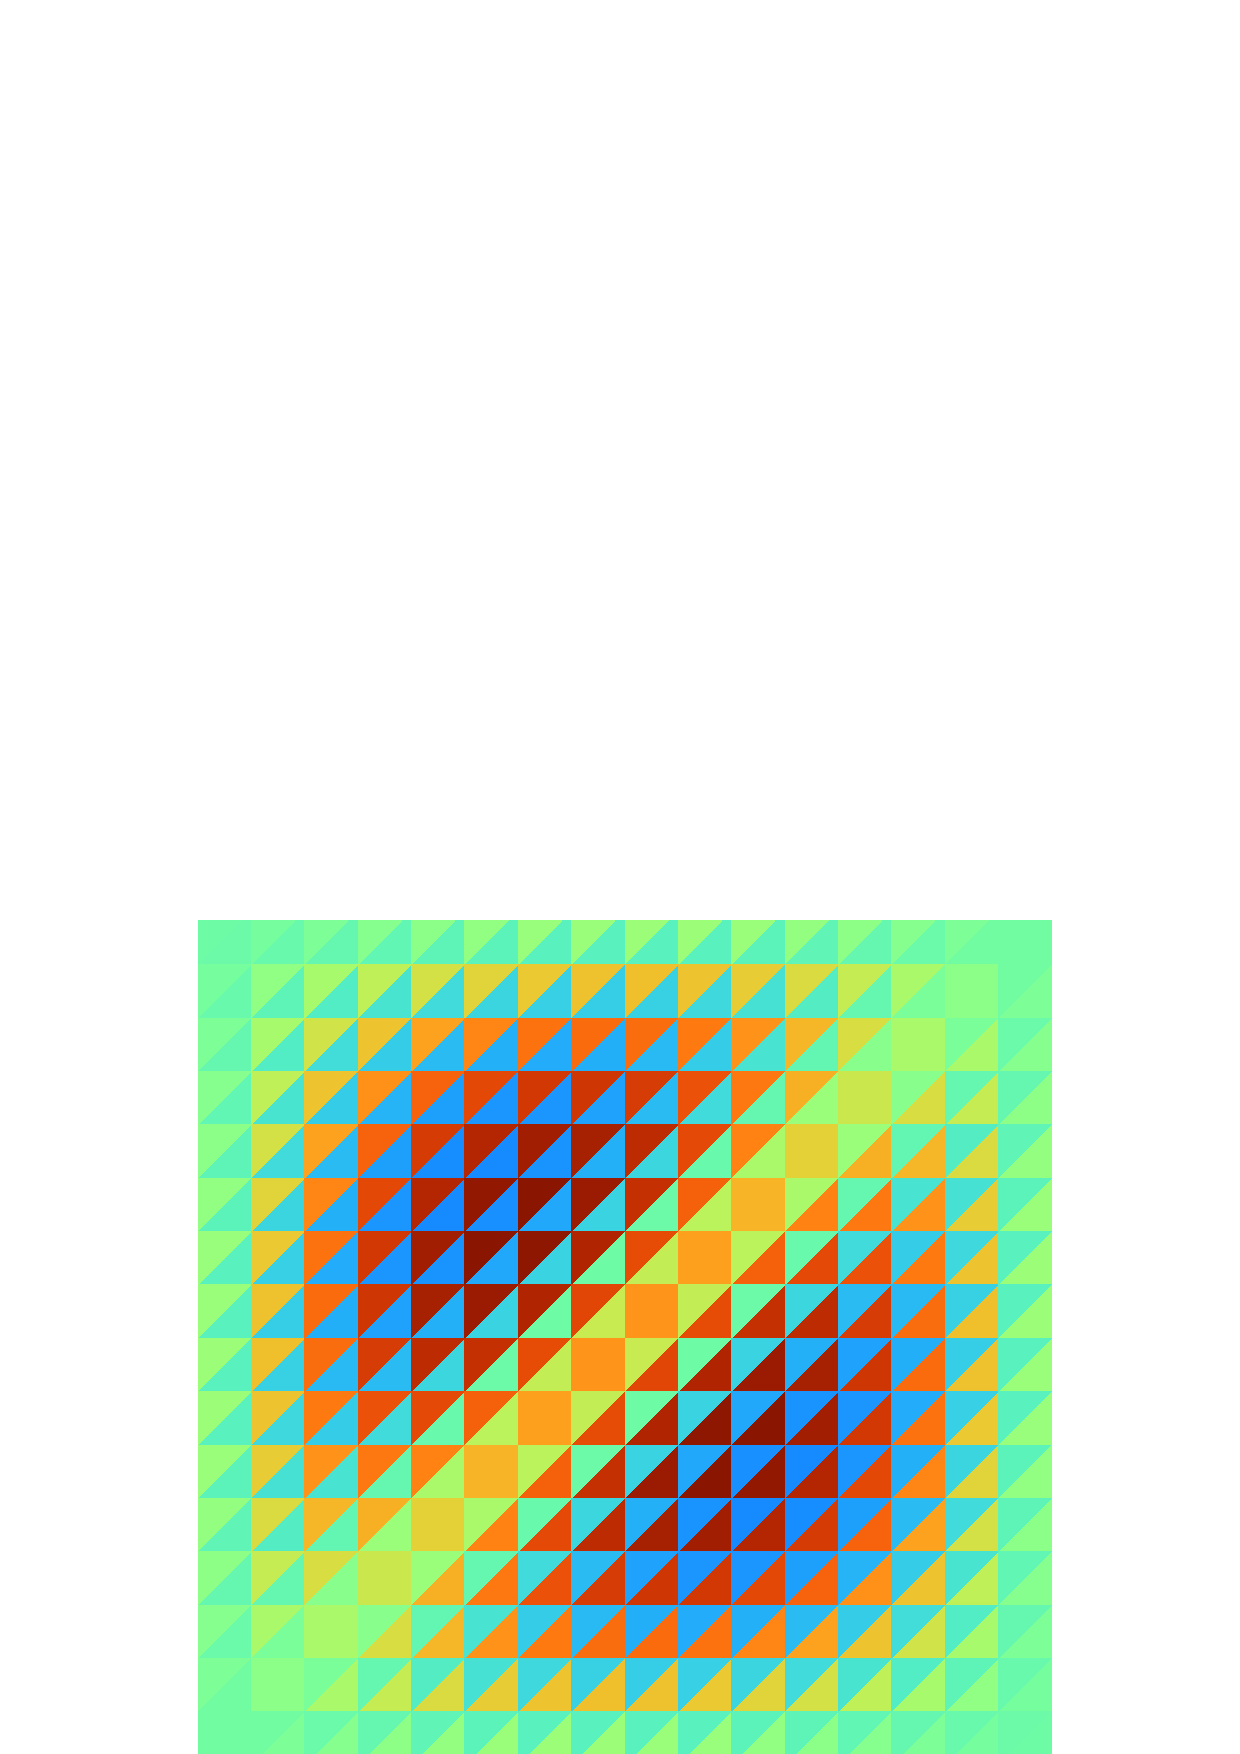
\includegraphics[width=\twofigs]{rognes/CG}}
%%  {\label{rognes:fig:rt} \includegraphics[width=\twofigs]{rognes/RT}}
%%  \caption{The scalar variable approximation $u_h$ for two choices
%%    of mixed finite element spaces for the mixed Laplacian. The data
%%    are as defined immediately above~\eqref{rognes:eq:mixedlaplace}.
%%    The element spaces are $\rognesvectorcg{1}{2} \times \rognesdg{0}$
%%    in~\subref{rognes:fig:cg} and $\rognesrt{1} \times \rognesdg{0}$
%%    in~\subref{rognes:fig:rt}. (The scales are less relevant for the
%%    current purpose and have therefore been
%%    omitted.)}
%%  \label{rognes:fig:example}
%%\end{figure}
\begin{figure}
\bwfig
  \centering
  \subfloat[Bad approximation]{\label{rognes:fig:cg} 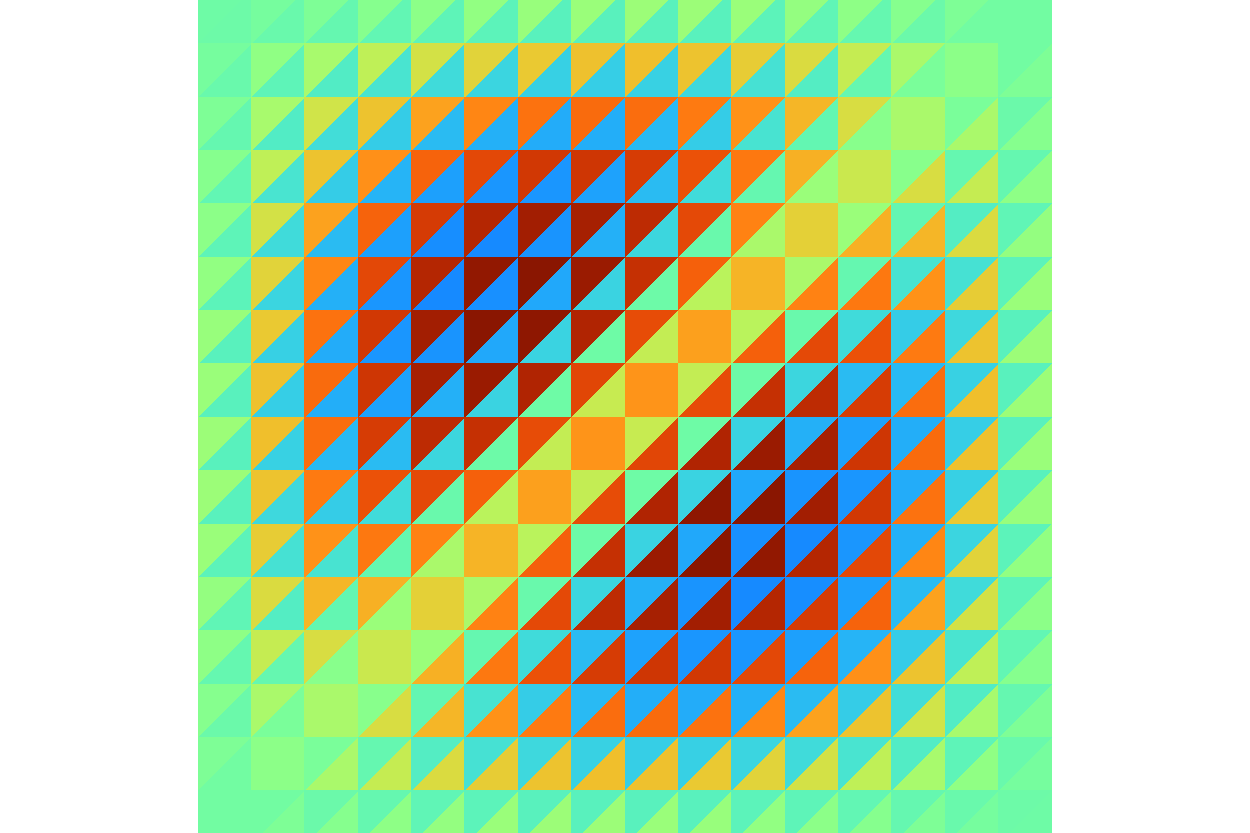
\includegraphics[width=\twofigs]{chapters/rognes/pdf/CG.pdf}}
  \subfloat[Good approximation]{\label{rognes:fig:rt} \includegraphics[width=\twofigs]{chapters/rognes/pdf/RT.pdf}}
  \caption{The scalar variable approximation $u_h$ for two choices
    of mixed finite element spaces for the mixed Laplacian. The data
    are as defined immediately above~\eqref{rognes:eq:mixedlaplace}.
    The element spaces are $\rognesvectorcg{1}{2} \times \rognesdg{0}$
    in~\subref{rognes:fig:cg} and $\rognesrt{1} \times \rognesdg{0}$
    in~\subref{rognes:fig:rt}. (The scales are less relevant for the
    current purpose and have therefore been
    omitted.)}
  \label{rognes:fig:example}
\end{figure}

The above two alternatives give unsatisfactory results because the
discretizations defined by the element spaces are both unstable. A
stable low order element pairing is the combination of the lowest
order Raviart--Thomas elements and the space of piecewise
constants~\citep{RaviartThomas1977}. The corresponding $u_h$
approximation is plotted in
Figure~\ref{rognes:fig:example}\subref{rognes:fig:rt}. This
approximation looks qualitatively correct.

The reason for the instabilities of the first two choices, and the
stability of the third choice, may not be immediately obvious. The
goal of this chapter is to construct a framework that automates this
stability identification procedure, by characterizing the stability
properties of a finite element discretization automatically and
accurately.  We will return to this example in
Section~\ref{rognes:sec:examples} where we give a more careful
characterization of the stability properties of the above sample
elements.

\section{Discrete stability}

In order to automatically characterize the stability of a
discretization, we need a precise definition of discrete stability and
preferably conditions for such to hold. In this section,
the \babuska{} and Brezzi stability conditions are described and
motivated in the general abstract setting. The material presented here
is largely taken from the classical references~\citet{Babuvska1972/73,
Brezzi1974, BrezziFortin1991}.

For a Hilbert space $W$, we denote the norm on $W$ by
$\|\cdot\|_{W}$ and the inner product by $\langle \cdot, \cdot
\rangle_{W}$. Assume that $\rognesc$ is a symmetric, bilinear
form on $W$ and that $L$ is a continuous, linear form on $W$. We will
consider the following canonical variational problem: find $u \in W$
such that
\begin{equation}
  \label{rognes:eq:canonical}
  \rognesc(u, v) = L(v) \quad \foralls v \in W.
\end{equation}
Assume that $\rognesc$ is continuous; that is, there exists a positive
constant $C$ such that
\begin{equation}
  |\rognesc(u, v)| \leqslant C \, \|u\|_{W} \|v\|_{W}
  \quad \foralls u, v \in W.
\end{equation}
If additionally there exists a positive constant $\gamma$ such that
\begin{equation}
  \rognesc(u, u) \geqslant \gamma \|u\|_{W}^2,
\end{equation}
the form $\rognesc$ is by definition coercive. This is indeed the case
for many variational formulations of partial differential equations
arising from standard minimization problems. On the other hand, for
many constrained minimization problems, such as those giving rise to
saddle point problems, the corresponding $\rognesc$ is not coercive.
Fortunately, the coercivity condition is sufficient, but not
necessary. A weaker condition suffices: there exists a positive
constant $\gamma$ such that
\begin{equation}
  \label{rognes:eq:infsup}
  0 < \gamma = \inf_{0 \not = u \in W} \sup_{0 \not = v \in W}
  \frac{|\rognesc(u,  v)|}{\|u\|_{W}\|v\|_{W}}.
\end{equation}
If the continuous $\rognesc$ satisfies~\eqref{rognes:eq:infsup}, there
exists a unique $u \in W$
solving~\eqref{rognes:eq:canonical}~\citep{Babuvska1972/73}.
\index{Ladyzhenskaya--\babuska{}--Brezzi conditions}
\index{LBB conditions}

Now, we turn to consider discretizations
of~\eqref{rognes:eq:canonical}. Let $W_h \subset W$ be a finite
dimensional subspace, and consider the discrete problem: find $u_h \in
W_h$ such that
\begin{equation}
  \label{rognes:eq:discrete}
  \rognesc(u_h, v) = L(v) \quad \foralls v \in W_h.
\end{equation}
For the discrete system to be well-posed, analogous conditions as for
the continuous case must be satisfied. Note that $\rognesc$ restricted
to $W_h$ is continuous \emph{a~fortiori}. However, the discrete
analogue of~\eqref{rognes:eq:infsup} does not trivially hold. In order
to guarantee that~\eqref{rognes:eq:discrete} has a unique solution, we
must also have that there exists a positive constant $\gamma_0$ such
that
\begin{equation}
  \label{rognes:eq:infsup:discrete}
  0 < \gamma_0 \leqslant \gamma_h = \inf_{0 \not = u \in W_h} \sup_{0
    \not = v \in W_h} \frac{|\rognesc(u, v)|}{\|u\|_{W}\|v\|_{W}}.
\end{equation}
Moreover, in order to have uniform behavior in the limit as $h
\rightarrow 0$, we must have that $\gamma_h \geqslant \gamma_0 > 0$ for all
$h > 0$; that is, that $\gamma_h$ is bounded from below independently
of $h$~\citep{Babuvska1972/73}.

The condition~\eqref{rognes:eq:infsup:discrete} has a simple
interpretation in the linear algebra perspective. Taking a basis
$\{\phi_i \}_{i=1}^n$ for $W_h$, in combination with the Ansatz $u_h =
u_j \phi_j$, we obtain the standard matrix formulation
of~\eqref{rognes:eq:discrete}:
\begin{equation}
  C_{ij} u_j = L(\phi_i) \quad i = 1, \dots, n,
\end{equation}
where $C_{ij} = c(\phi_j, \phi_i)$. The Einstein notation, in which
summation over repeated indices is implied, has been used here. This
system will have a unique solution if the matrix $C$ is non-singular,
or equivalently, if the eigenvalues of $C$ are nonzero. In the
special case where $c$ is coercive, all eigenvalues will in fact be
positive. Moreover, we must ensure that the generalized eigenvalues
(generalized with respect to the inner product on $W$) do not approach
zero as $h \rightarrow 0$. This is precisely what is implied by the
condition~\eqref{rognes:eq:infsup:discrete}.

\subsection{Stability conditions for saddle point problems}
\index{saddle point problem}

We now turn to consider the special case of abstract saddle point
problems. In this case, the stability
condition~\eqref{rognes:eq:infsup:discrete} can be rephrased in an
alternative, but equivalent form.

Assume that $V$ and $Q$ are Hilbert spaces, that $a$ is a continuous,
symmetric, bilinear form on $V \times V$, that $b$ is a continuous,
bilinear form on $V \times Q$, and that $L$ is a continuous linear
form on $V \times Q$. A saddle point problem has the following
canonical form: find $u
\in V$ and $p \in Q$ such that
\begin{equation}
    \label{rognes:eq:saddlepoint}
    a(u, v) + b(v, p) + b(u, q) = L((v, q))
    \quad \foralls v \in V, q \in Q.
\end{equation}
The system~\eqref{rognes:eq:saddlepoint} is clearly a special case
of~\eqref{rognes:eq:canonical} with the following identifications: let
$W = V \times Q$, endow the product space with the norm $\|(v,
q)\|_{W} = \|v\|_{V} + \|q\|_{Q}$, and label
\begin{equation}
  c((u, p), (v, q)) = a(u, v) + b(v, p) + b(u, q).
\end{equation}
Assuming that the condition~\eqref{rognes:eq:infsup} is satisfied, the
above system admits a unique solution $(u, p) \in V \times Q$.

As in the general case, we aim to
discretize~\eqref{rognes:eq:saddlepoint}, but now using a pair of
conforming finite element spaces $V_h$ and $Q_h$. Letting $W_h = V_h
\times Q_h$, we obtain the following special form
of~\eqref{rognes:eq:discrete}: find $u_h \in V_h$ and $p_h \in Q_h$
satisfying:
\begin{equation}
    \label{rognes:eq:saddlepoint:discrete}
    a(u_h, v) + b(v, p_h) + b(u_h, q) = L((v, q))
    \quad \foralls v \in V_h, q \in Q_h.
\end{equation}
Again, the well-posedness of the discrete problem follows from the
general theory. Applying the definition
of~\eqref{rognes:eq:infsup:discrete} to~\eqref{rognes:eq:saddlepoint},
we define the \babuska{} constant $\gamma_h$:
\begin{equation}
  \label{rognes:eq:Babuska}
  \gamma_h = \inf_{0 \not = (u, p) \in W_h} \sup_{0 \not = (v, q) \in W_h}
  \frac{|a(u, v) + b(v, p) + b(u, q)|} {(\|u\|_{V} + \|p\|_{Q})
    (\|v\|_{V} + \|q\|_{Q})}
\end{equation}
In particular, the discrete problem is well-posed if the \babuska{}
stability condition holds; namely, if $\gamma_h \geqslant \gamma_0 >
0$ for any $h > 0$.
\index{Babu\v{s}ka condition}

%%% --------------------------------------------------------------

The previous deliberations simply summarized the general theory
applied to the particular variational form defined
by~\eqref{rognes:eq:saddlepoint}. However, the special structure
of~\eqref{rognes:eq:saddlepoint} also offers an alternative
characterization. The single \babuska{} stability condition can be
split into a pair of stability conditions as
follows~\citep{Brezzi1974}. Define
\begin{align}
  \label{rognes:eq:brezzi:coercivity}
  \alpha_h =
  \inf_{0 \not = u \in Z_h}
  \sup_{0 \not = v \in Z_h}
  \frac{a(u, v)}{\|u\|_{V} \|v\|_{V}} , \\
  \label{rognes:eq:brezzi:infsup}
  \beta_h =
  \inf_{0 \not = q \in Q_h}
  \sup_{0 \not = v \in V_h}
  \frac{b(v, q)}
       {\|v\|_{V} \|q\|_{Q}},
\end{align}
where
\begin{equation}
  Z_h = \{ v \in V_h \, | \, b(v, q) = 0 \quad \foralls q \in Q_h\}.
\end{equation}
We shall refer to $\alpha_h$ as the Brezzi coercivity constant and
$\beta_h$ as the Brezzi inf-sup constant. The Brezzi stability
conditions state that these must stay bounded above zero for all $h >
0$. The Brezzi conditions are indeed equivalent to the \babuska{}
condition~\citep{Brezzi1974}. However, for a specific saddle point
problem and a given pair of function spaces, it might be easier to
verify the two Brezzi conditions than the single \babuska{} condition.
In summary, these conditions enable a concise characterization of the
stability of discretizations of saddle point problems.
\begin{definition}
  \label{rognes:def:stable}
  A family of finite element discretizations $\{V_h \times Q_h\}_h$
  is \emph{stable in $V \times Q$} if the Brezzi coercivity and
  inf-sup constants $\{ \alpha_h \}_h $ and $\{ \beta_h \}_h$ (or
  equivalently the \babuska{} inf-sup constants $\{ \gamma_h \}_h$)
  are bounded from below by a positive constant independent of $h$.
\end{definition}
Throughout this chapter, the term \emph{a family of discretizations}
refers to a collection of finite element discretizations parametrized
over a family of meshes.
\index{Brezzi inf-sup condition}
\index{Brezzi coercivity condition}

There are families of discretizations that are not stable in the sense
defined above, but possess a certain reduced stability. For a pair
$V_h \times Q_h$, we can define the space of spurious modes $N_h
\subseteq Q_h$:
\begin{equation}
  N_h
  = \{q \in Q_h \, | \; b(v, q) = 0 \quad
  \foralls v \in V_h\}.
\end{equation}
It can be shown that the Brezzi inf-sup constant is positive if and
only if there are no nontrivial spurious modes; that is, if $N_h = \{
0 \}$~\citep{Qin1994}. On the other hand, if $N_h$ is nontrivial, one
may, loosely speaking, think of the space $Q_h$ as a bit too large.
In that case, it may be natural to replace $Q_h$ by the reduced space
$N_h^{\perp}$, the orthogonal complement of $N_h$ in $Q_h$. This idea
motivates the definition of the reduced Brezzi inf-sup constant,
relating to the stability of $V_h \times N_h^{\perp}$:
\begin{equation}
  \label{rognes:eq:reduced:infsup}
  \tilde \beta_h =
  \inf_{0 \not = q \in N_h^{\perp}}
  \sup_{0 \not = v \in V_h}
  \frac{b(v, q)}
       {\|v\|_{V} \|q\|_{Q}},
\end{equation}
and the definition of reduced stable below. By definition, $\tilde
\beta_h \not = 0$. The identification of reduced stable
discretizations can be interesting from a theoretical
viewpoint. Further, such could be used for practical purposes after a
filtration of the spurious modes.
\begin{definition}
  \label{rognes:def:reduced_stable}
  A family of discretizations $\{V_h \times Q_h\}_h$ is \emph{reduced
  stable in $V \times Q$} if the Brezzi coercivity constants
  $\{\alpha_h\}_h$ and the reduced Brezzi inf-sup constants
  $\{ \tilde \beta_h \}_h$ are bounded from below by a positive
  constant independent of $h$.
\end{definition}
\index{reduced discrete stability}

\section{Eigenvalue problems associated with saddle point stability}

For a given variational problem, the Brezzi conditions provide a
method to inspect the stability of a family of conforming
discretizations, defined relative to a family of meshes. However, it
seems hardly feasible to automatically verify these conditions in
their current form. Fortunately and as we shall see in this section,
there is an alternative characterization of the \babuska{} and Brezzi
constants: each stability constant will be related to the smallest (in
modulus) eigenvalue of a certain eigenvalue problem. The automatic
testing of the stability of a given discretization family can
therefore be based on the computation and inspection of certain
eigenvalues.

We begin by considering the \babuska{} inf-sup constant for the
element pair $V_h \times Q_h$. It can be easily seen that
the \babuska{} inf-sup constant $\gamma_h = |\lambda_{\min}|$ where
$\lambda_{\min}$ is the smallest in modulus eigenvalue of the
generalized eigenvalue problem~\citep{ArnoldRognes2009, Malkus1981}:
find $0 \not = (u_h, p_h) \in V_h \times Q_h$ and $\lambda \in \R$
such that
\begin{equation}
  \label{rognes:eq:eigenvalue:babuska}
  a(u_h, v) + b(v, p_h) + b(u_h, q)
  = \lambda
  \left (\langle u_h, v \rangle_{V} + \langle p_h, q \rangle_{Q} \right )
  \quad \foralls v \in V, q \in Q.
\end{equation}

By the same arguments, the Brezzi coercivity constant $\alpha_h$ is
the smallest in modulus eigenvalue of the following generalized
eigenvalue problem: find $0 \not = u_h \in Z_h$ and $\lambda \in \R$
satisfying
\begin{equation}
  \label{rognes:eq:eigenvalue:kernel}
  a(u_h, v) = \lambda \langle u_h, v \rangle_{V}
\end{equation}
For the spaces $V_h$ and $Q_h$, a basis is normally known. For $Z_h$
however, this is usually not the case. (If it had been, the space
$Z_h$ might have been better to compute with in the first place.)
Therefore, the eigenvalue problem~\eqref{rognes:eq:eigenvalue:kernel}
is not that easily constructed in practice.

Instead, one may consider an alternative generalized eigenvalue
problem: find $0 \not = (u_h, p_h) \in V_h \times Q_h$ and $\lambda
\in \R$ satisfying
\begin{equation}
  \label{rognes:eq:eigenvalue:coercivity}
  a(u_h, v) + b(v, p_h) + b(u_h, q) = \lambda \langle u_h, v \rangle_{V}
\end{equation}
It can be shown that the smallest in modulus eigenvalue of the above
eigenvalue problem and the smallest in modulus eigenvalue
of~\eqref{rognes:eq:eigenvalue:kernel}
agree~\citep{ArnoldRognes2009}. Therefore $\alpha_h =
|\lambda_{\min}|$ when $\lambda_{\min}$ is the smallest in modulus
eigenvalue of~\eqref{rognes:eq:eigenvalue:coercivity}. The eigenvalue
problem~\eqref{rognes:eq:eigenvalue:coercivity} involves the spaces
$V_h$ and $Q_h$ and is therefore more tractable. One word of caution
however: if there exists a $q \in Q_h$ such that $b(v, q) = 0$ for all
$v \in V_h$, then any $\lambda$ is an eigenvalue
of~\eqref{rognes:eq:eigenvalue:coercivity}. Thus, the
problem~\eqref{rognes:eq:eigenvalue:coercivity} is ill-posed if such
$q$ exists. The case where such $q$ exists is precisely the case where
the Brezzi inf-sup constant is zero.

Finally, the Brezzi inf-sup constant $\beta_h$ is the square root of
the smallest eigenvalue $\lambda_{\min}$ of the following eigenvalue
problem~\citep{Malkus1981, Qin1994}: find $0 \not = (u_h, p_h) \in V_h
\times Q_h$ and $\lambda \in \R$ satisfying
\begin{equation}
  \label{rognes:eq:eigenvalue:infsup}
  \langle u_h, v \rangle_{V} + b(v, p_h) + b(u_h, q) = - \lambda
  \langle p_h, q \rangle_{Q}
\end{equation}
The eigenvalues of~\eqref{rognes:eq:eigenvalue:infsup} are all
non-negative. Any eigenvector associated with a zero eigenvalue
corresponds to a spurious mode. Further, the square root of the
smallest nonzero eigenvalue will be the reduced Brezzi inf-sup
constant~\citep{Qin1994}.

\section{Automating the stability testing}
\label{rognes:sec:automation}

The mathematical framework is now in place. For a given variational
formulation, given inner product(s), and a family of function spaces,
the eigenvalue problem~\eqref{rognes:eq:eigenvalue:babuska} or the
problems~\eqref{rognes:eq:eigenvalue:coercivity}
and~\eqref{rognes:eq:eigenvalue:infsup} can be used to numerically
check stability. The eigenvalue
problem~\eqref{rognes:eq:eigenvalue:infsup} applied to the Stokes
equations was used in this context by
\citet{Qin1994} and \citet{ChapelleBathe1993}. A fully automated approach
has not been previously available though. This is perhaps not so strange,
as an automated approach would be rather challenging to implement within
many finite element libraries. However, DOLFIN provides ample and
suitable tools for this task. In particular, the \ufl{} form language,
the collection of finite element spaces supported by \fiat{}/\ffc{}, and
the available \slepc{} eigenvalue solvers provide the required functionality.

The definition of an abstract saddle point
problem~\eqref{rognes:eq:saddlepoint} and the definition of stability
of discretizations of such, Definition~\ref{rognes:def:stable},
provide a natural starting point. Based on these definitions, the
testing of stability relies on the following input.
\begin{itemize}
\item The bilinear forms $a$ and $b$ defining a variational
  saddle point problem.
\item The function spaces $V$ and $Q$ through the inner products
  $\langle \cdot, \cdot \rangle_{V}$ and $\langle \cdot, \cdot
  \rangle_{Q}$.
\item A family of finite element function spaces $\{W_h\}_h = \{V_h
  \times Q_h \}_h$ parametrized over the mesh size $h$.
\end{itemize}
We pause to remark that since~\eqref{rognes:eq:saddlepoint} is a
special case of the canonical form~\eqref{rognes:eq:canonical}, one
may consider the
\babuska{} constant only. However, for the analysis of saddle point
problems, the separate behavior of the individual Brezzi constants
may be interesting. For this reason, we focus on the Brezzi stability
conditions and the decomposed variational form here.

The following strategy presents itself naturally in order to attempt
to characterize the stability of a discretization family. With the
above information, one can proceed in the following steps
\begin{enumerate}
\item For each function space $W_h$, construct the eigenvalue problems
  associated with the Brezzi conditions
\item Solve the eigenvalue problems and identify the appropriate
  eigenvalues corresponding to the Brezzi constants.
\item Based on the behavior of the Brezzi constants with respect to
  $h$, the discretization family should be classified,
  see~Definitions~\ref{rognes:def:stable}
  and~\ref{rognes:def:reduced_stable}, as
  \begin{enumerate}
  \item Stable
  \item Unstable
  \item Unstable, but reduced stable
  \end{enumerate}
\end{enumerate}

The above strategy is implemented in the automated stability condition
tester \rognesascot{}~\citep{Rognes2009}. \rognesascot{} is a
\rognespython{} module dependent on DOLFIN compiled with
\slepc{}. It is designed to automatically evaluate the stability of a
discretization family, and in particular, the stability of mixed
finite element methods for saddle point problems. \rognesascot{} can
be imported as any \rognespython{} module:
\begin{python}
from ascot import *
\end{python}
The remainder of this section describes how the afore described
strategy is implemented in \rognesascot{}. Emphasis is placed on the
form of the input, the construction and solving of the eigenvalue
problems, and the classification of stability based on the stability
constants.

Before continuing however, it is necessary to point out a limitation
of the numerical testing. The mathematical definition of stability is
indeed based on taking the limit as $h \rightarrow 0$. However, it is
hardly feasible to examine an infinite family of function spaces
$\{W_h\}_{h \in \R^{+}}$ numerically. In practice, one can only
consider a finite set of spaces $\{W_{h_i}\}_{i \in (0, \dots,
N)}$. Therefore, this strategy can only give numerical evidence, which
must be interpreted using appropriate heuristics.

\subsection{Defining input}
\label{rognes:subsec:input}

\rognesascot{} relies on the variational form language defined by \ufl{} and
DOLFIN for the specification of forms, inner products and function
spaces.  In order to illustrate, we take the discrete mixed Laplacian
introduced in~\eqref{rognes:eq:mixedlaplace:discrete} as an example.

First and foremost, consider the specification of the forms $a$ and
$b$. Recall that discrete saddle point stability is not a property
relating to a single set of function spaces, but rather a property
relating to a family of function spaces. In the typical DOLFIN
approach, forms are specified in terms of basis functions on a single
function space. For our purposes, this seems like a less ideal
approach. Instead, to be able to specify the forms independently of
the function spaces, we can take advantage of the \rognespython{}
$\lambda$ functionality. For the mixed Laplacian, the forms $a$ and
$b$ read $a = a(u, v) = \langle u, v \rangle$ and $b = b(v, q) =
\langle \Div v, q \rangle$. These should be specified as
\begin{python}
# Define a and b forms:
a = lambda u, v: dot(u, v)*dx
b = lambda v, q: div(v)*q*dx
\end{python}
The above format is advantageous as it separates the definition of the
forms from the function spaces. Hence, the user needs not specify
basis functions on each of the separate function
spaces: \rognesascot{} handles the initialization of the appropriate
basis functions.

Second, the inner products $\langle \cdot, \cdot \rangle_V$ and
$\langle \cdot, \cdot \rangle_Q$ must be provided. The inner products
are bilinear forms and can therefore be viewed as a special case of
the above. For the mixed Laplacian, the appropriate inner products are
$\langle u, v \rangle_{\Div} = \langle u, v \rangle + \langle \Div u,
\Div v \rangle$ and $\langle p, q \rangle_0 = \langle p, q \rangle$. The
corresponding code reads
\begin{python}
# Define inner products:
Hdiv = lambda u, v: (dot(u, v) + div(u)*div(v))*dx
L2 = lambda p, q: dot(p, q)*dx
\end{python}

Third, the function spaces have to be specified. In particular, a list
of function spaces corresponding to a set of meshes should be defined.
For the testing of the mixed function space consisting of continuous
piecewise linear vector fields $\rognesvectorcg{1}{2}$, combined with
continuous piecewise linears $\rognescg{1}$, for a set of diagonal
triangulations of the unit square, one can do as follows:
\begin{python}
# Construct a family of mixed function spaces
meshsizes = [2, 4, 6, 8, 10]
meshes = [UnitSquare(n, n) for n in meshsizes]
W_hs = [VectorFunctionSpace(mesh, "Lagrange", 1)*FunctionSpace(mesh, "Lagrange", 1)
        for mesh in meshes]
\end{python}
Note that the reliability of the computed stability characterization
increases with the number of meshes and their refinement level.

The stability of the above can now be tested. The main entry point
function provided by \rognesascot{} is \emp{test\_stability}. This
function takes three arguments: a list of forms, a list of inner
products and a list of function spaces:
\begin{python}
result = test_stability((a, b), (Hdiv, L2), W_hs)
\end{python}
A \emp{StabilityResult} is returned.  The instructions carried out by
this function and the properties of the \emp{StabilityResult} are
described in the subsequent paragraphs.

\subsection{Constructing and solving eigenvalue problems}

For the testing of saddle point problems, specified by the two forms
$a$ and $b$, it is assumed that the user wants to check the Brezzi
conditions. In order to test these conditions, the Brezzi constants;
that is, the Brezzi coercivity and Brezzi inf-sup constants, must be
computed for each of the function spaces. \rognesascot{} provides
functionality for the computation of these constants: the functions
\emp{compute\_brezzi\_coercivity} and
\emp{compute\_brezzi\_infsup}.

Let us take a closer look at the implementation
of \emp{compute\_brezzi\_infsup}. The input consists of the form $b$,
the inner products $m$ and $n$, and a function space $W_h$ (and
optionally, an essential boundary condition \emp{bc}). The aim is to
construct the eigenvalue problem given
by~\eqref{rognes:eq:eigenvalue:infsup} and then solve this problem
efficiently. To accomplish this, the basis functions on the function
space $W_h$ are defined first. The left and right-hand sides of the
eigenvalue problems are specified through the forms defined
by~\eqref{rognes:eq:eigenvalue:infsup}. These forms are sent to an
\emp{EigenProblem}, and the resulting eigenvalues are then
used to initialize an \emp{InfSupConstant}. The
\emp{InfSupConstant} class is a part of the
characterization machinery and will be discussed further in the next
subsection.
\begin{python}
def compute_brezzi_infsup(b, (m, n), W, bc=None):
    """
    For a given form b: V x Q \rightarrow \R and inner products m and
    n defining V and Q respectively and a function space W = V_h x
    Q_h, compute the Brezzi inf-sup constant.
    """
    # Define forms for eigenproblem
    (u, p) = TrialFunctions(W)
    (v, q) = TestFunctions(W)
    lhs = m(u, v) + b(v, p) + b(u, q)
    rhs = - n(p, q)

    # Get parameters
    params = ascot_parameters["brezzi_infsup"]
    num = ascot_parameters["number_of_eigenvalues"]

    # Compute eigenvalues
    eigenvalues = EigenProblem(lhs, rhs, params, bc).solve(num)
    return InfSupConstant(W.mesh().hmax(), eigenvalues, operator=sqrt)
\end{python}
The computation of the Brezzi coercivity constant takes a virtually
identical form, only differing in the definition of the left and
right-hand sides (\emp{lhs} and \emp{rhs}). If only a single form $c$
and a single inner product $m$ is specified, the \babuska{} condition
is tested by similar constructs.

The \emp{EigenProblem} class is a simple wrapper class for the
\dolfin{} \emp{SLEPcEigenSolver}, taking either a single form,
corresponding to a standard eigenvalue problem, or two forms,
corresponding to a generalized eigenvalue problem. The eigenvalue
problems generated by the \babuska{} and Brezzi conditions are all
generalized eigenvalue problems. For both the Brezzi conditions, the
right-hand side matrix will always be singular. The left-hand side
matrix may or may not be singular depending on the discretization. For
the \babuska{} conditions, the right-hand side matrix should never be
singular, however the left-hand side matrix may be.

\slepc{} provides a collection of eigenvalue solvers that can handle
generalized, possibly singular eigenvalue
problems~\citep{HernandezRomanVidal2005,
HernandezRomanRomeroEtAl2009}. The type of eigenvalue solver can be
specified through the \dolfin{} parameter interface. For our purposes,
two solver types are particularly relevant: the LAPACK and the
Krylov-Schur solvers.  The LAPACK solver is a direct method. This
solver is very robust. However, it computes all of the eigenvalues,
and it is thus only suited for relatively small problems. In contrast,
the Krylov-Schur method offers the possibility of only computing a
given number of eigenvalues. Since the Brezzi constants are related to
the eigenvalue closest to zero, it seems meaningful to only compute
the eigenvalue of smallest magnitude. This solver is therefore set as
the default solver type in
\rognesascot. Unfortunately, the Krylov-Schur solver is less robust
for singular problems: it may fail to converge. A partial remedy may
be to apply a shift-and-invert spectral transform with an appropriate
shift factor to the eigenvalue problem. For more details on spectral
transformations in \slepc{}, see
\citet{HernandezRomanRomeroEtAl2009}. \rognesascot{} applies a
shift-and-invert transform with a small shift factor by default for
the Brezzi and \babuska{} inf-sup problems.

\subsection{Characterizing the discretization}

After the eigenvalues and thus the stability constants are computed
for the family of function spaces, all that remains is to interpret
these constants. \rognesascot{} provides three classes intended to represent
and interpret the behavior of the stability constants:
\emp{InfSupConstant}, \emp{InfSupCollection} and
\emp{StabilityResult}.

An \emp{InfSupConstant} represents a single inf-sup constant. It is
initialized using a mesh size $h$, a set of values, and an optional
operator. The values typically correspond to the computed
eigenvalues. If supplied, the operator is applied to the eigenvalues.
For instance, \rognesascot{} supplies a square root operator when
computing the Brezzi inf-sup constant. The object can return the
inf-sup constant and, if computed, the reduced inf-sup constant and
the number of zero eigenvalues. The latter two items are most useful
for careful analysis purposes.

A collection of \emp{InfSupConstant}s forms
an \emp{InfSupCollection}. An \emp{InfSupCollection}'s main purpose is
to identify whether or not the stability condition associated with the
inf-sup constants holds. The method \emp{is\_stable} returns a boolean
answer. The stability condition will not hold if any of the inf-sup
constants is zero, and it will probably not hold if the inf-sup
constants seem to decay with the mesh size $h$.  The rate of decay
$r_i$ between two subsequent constants $c_i$ and $c_{i+1}$ is defined
as:
\begin{equation}
  r_i = \frac{\log_2(c_i) - \log_2(c_{i+1})}{\log_2(h_i) -
    \log_2(h_{i+1})}
\end{equation}
where $h_i$ is the corresponding mesh size. Currently, \rognesascot{}
classifies a discretization as stable if there are no singularities
(no zero eigenvalues for all meshes), and the decay rates are below
$1$ and consistently decrease, or the rate corresponding to the finest
mesh is less than a heuristically chosen small number.

Finally, the \emp{StabilityResult} class holds a list of possibly
several \emp{InfSupCollections}, each corresponding to a separate
inf-sup condition, such as the Brezzi coercivity and the Brezzi
inf-sup condition. The \emp{StabilityResult} identifies a
discretization as stable if all stability conditions are satisfied,
and as unstable otherwise.

\section{Examples}
\label{rognes:sec:examples}

In this section, we apply the automated stability testing framework to
two classical saddle point problems: the mixed Laplacian and the
Stokes equations. The behavior of the various mixed finite elements
observed in Section~\ref{rognes:sec:motivation} will be explained and
classical analytical results reproduced. The complete code is
available from the demo directory of the \rognesascot{} module.

\subsection{Mixed Laplacian}
\index{Poisson's equation!mixed finite element discretization}

We can now return to the mixed Laplacian example described in
Section~\ref{rognes:sec:motivation} and inspect the Brezzi stability
properties of the element spaces involved, namely
$\rognesvectorcg{1}{2} \times \rognescg{1}$, $\rognesvectorcg{1}{2}
\times \rognesdg{0}$ and $\rognesrt{1} \times \rognesdg{0}$. The
example considered a family of diagonal triangulations of the unit
square. The complete code required to test the stability of the first
discretization family was presented piecewise in
Section~\ref{rognes:subsec:input}. The stability result can be
inspected as follows:
\begin{python}
print result
for condition in result.conditions:
    print condition
\end{python}
The following output appears:
\begin{progoutput}
<Mixed element: (<Mixed element: (<CG1 on a <triangle of degree 1>>,
<CG1 on a <triangle of degree 1>>)>, <CG1 on a <triangle of degree 1>>)>

Not computing Brezzi coercivity constants because of singularity
Discretization family is: Unstable. Singular. Decaying.

InfSupCollection: beta_h
singularities =  [2, 2, 2, 2, 2]
reduced =        [0.56032, 0.35682, 0.24822, 0.18929, 0.15251]
rates  =         [0.651, 0.895, 0.942, 0.968]

Empty InfSupCollection: alpha_h
\end{progoutput}
\rognesascot{} characterizes this discretization family as
unstable. For the Brezzi inf-sup eigenvalue problems, there are 2 zero
eigenvalues for each mesh. Hence, the Brezzi inf-sup constant is zero,
and moreover, the element matrix will be singular. This is precisely
what we observed in the introductory example: there was no solution to
the discrete system of equations. Moreover, the reduced inf-sup
constant is also decaying with the mesh size at a rate that seems to
be increasing towards $\mathcal{O}(h)$. So, there is no hope of
recovering a stable method by filtering out the spurious modes. Since
each Brezzi inf-sup constant is zero, the Brezzi coercivity eigenvalue
problems are not computationally well-posed, and thus these constants
have not been computed.

The second family of elements considered in
Section~\ref{rognes:sec:motivation} was the combination of continuous
piecewise linear vector fields and piecewise constants. Using the same
code as before, just replacing the finite element spaces, we obtain
the following results:
\begin{progoutput}
<Mixed element: (<Mixed element: (<CG1 on a <triangle of degree 1>>,
<CG1 on a <triangle of degree 1>>)>, <DG0 on a <triangle of degree 1>>)>
Discretization family is: Unstable. Decaying.

InfSupCollection: beta_h
values =         [0.96443, 0.84717, 0.71668, 0.60558, 0.51771]
rates  =         [0.187, 0.413, 0.586, 0.703]

InfSupCollection: alpha_h
values =         [1, 1, 1, 1, 1]
rates  =         [-1.35e-14, 6.13e-14, 3.88e-13, 4.05e-13]
\end{progoutput}
Look at the Brezzi inf-sup constants first. In this case, there are no
singular values, and hence the Brezzi inf-sup constants are
positive. However, the constants seem to decay with the mesh size at
increasing rates. Extrapolating, we can suppose that the constants
$\beta_h$ depend on the mesh size $h$ and decay towards zero with
$h$. \rognesascot{} accordingly labels the discretization as
unstable. Since there are no singular values, the Brezzi coercivity
problem is well-posed. The Brezzi coercivity constants have therefore
been computed. We see that the Brezzi coercivity constant is equal to
one for all of the meshes tested. This is also easily deduced: the
divergence of the velocity space is included in the pressure space and
hence the Brezzi coercivity constant is indeed one for all
meshes. Since neither constant is singular, we expect the discrete
system of equations to be solvable -- as we indeed saw in
Section~\ref{rognes:sec:motivation}. The problem with this method
hence only lies in the decaying Brezzi inf-sup constant. However, the
instability did indeed manifest itself in the discrete approximation
see~Figure~\ref{rognes:fig:example}\subref{rognes:fig:cg}.

Finally, we can inspect a stable method, namely the lowest order
Raviart--Thomas space combined with the space of piecewise constants:
\begin{progoutput}
<Mixed element: (<RT1 on a <triangle of degree 1>>,
<DG0 on a <triangle of degree 1>>)>
Discretization family is: Stable.

InfSupCollection: beta_h
values =         [0.97682, 0.97597, 0.97577, 0.97569, 0.97566]
rates  =         [0.00126, 0.000508, 0.000265, 0.000162]

InfSupCollection: alpha_h
values =         [1, 1, 1, 1, 1]
rates  =         [5.6e-11, 1.39e-08, 1.64e-08, 2.24e-07]
\end{progoutput}
\rognesascot{} characterizes this mixed element method as stable. It
is indeed proven so \citep{RaviartThomas1977}. The Brezzi coercivity
constant is equal to $1$ for all meshes tested and hence bounded from
below. The Brezzi inf-sup constant definitely seems to be bounded from
below. The constant will actually converge to the value $\sqrt{2} \pi
(1 + 2 \pi^2)^{-1/2}$, see~\citet{ArnoldRognes2009}.  The satisfactory
result observed in
Figure~\ref{rognes:fig:example}\subref{rognes:fig:rt} is thus
agreement with the general theory.

\paragraph*{Caveat emptor.}

It is worth noting that the stability properties of some mixed
elements can vary dramatically. Here is one example: take the
combination of continuous linear vector fields and piecewise constants
for the mixed Laplacian. As we have seen above, this element family is
non-singular on the diagonal mesh family, but the Brezzi inf-sup
constants decay. However, if we inspect a family of criss-cross
meshes, specified in DOLFIN using
\begin{python}
meshes = [UnitSquare(n, n, "crossed") for n in meshsizes]
\end{python}
with the mesh sizes as before, the results are different:
\begin{progoutput}
Discretization family is: Unstable. Singular. Reduced stable.

InfSupCollection: beta_h
singularities = [4, 16, 36, 64, 100]
reduced =        [0.97832, 0.97637, 0.97595, 0.97579, 0.97572]
rates  =         [0.00288, 0.00106, 0.000543, 0.000328]
\end{progoutput}
For this mesh family, the Brezzi inf-sup constants are zero and thus
the method is singular. (In fact, there are $n^2$ spurious modes for
this element on this mesh \citep{Qin1994}.) However, the reduced
Brezzi inf-sup constants seem to be bounded from below, and so the
method could theoretically be stabilized by a removal of the spurious
modes. For a careful study of the stability of Lagrange elements for
the mixed Laplacian on various mesh families,
see~\citet{ArnoldRognes2009}.

The results may be more different than illustrated above. A truly
stable method will be stable for any admissible tessellation family,
but there are methods that are stable on some mesh families, but not
in general.  Therefore, if determining whether a mixed element is
appropriate or not, the discretization should be tested on more than a
single mesh family.

\subsection{Stokes}

\index{Stokes equations!mixed finite element discretization}

The Stokes equations is another classical and highly relevant saddle
point problem. For simplicity, we here consider the following discrete
formulation: find the velocity $u_h \in V_h$, and the pressure $p_h
\in Q_h$ such that
\begin{equation}
  \label{rognes:eq:stokes}
  \begin{split}
    \langle \Grad u_h, \Grad v \rangle + \langle \Div v, p_h \rangle &=
    \langle f, v \rangle
    \quad\quad \foralls v \in V_h, \\
    \langle \Div u_h, q \rangle &= 0
    \quad \foralls q \in Q_h.
  \end{split}
\end{equation}

The previous example demonstrated that it is feasible, even easy, to
test stability for any given family of discretizations. Taking this a
step further, we can generate a set of all available conforming
function spaces on a family of meshes, and test the stability of
each. With this aim in mind, \rognesascot{} provides some
functionality for creating combinations of mixed function spaces given
information on the value dimension of the spaces, the polynomial
degree, the meshes and the desired regularity. For instance, to
generate all available $H^1$-conforming vector fields of polynomial
degree between $1$ and $4$ matched with $L^2$-conforming functions of
polynomial degrees between $0$ and $3$ on a given set of meshes,
define
\begin{python}
specifications = {"value_dimensions": (2, 1),
                  "degrees": ((i,j) for i in range(1,5) for j in range(i)),
                  "spaces": ("H1", "L2")}
spaces = create_spaces(meshes, **specifications)
\end{python}

For the equations~\eqref{rognes:eq:stokes}, the Brezzi coercivity
condition always holds as long as $V_h$ does not contain the constant
functions. Therefore, it suffices to examine the Brezzi inf-sup
condition. For simplicity though, we here examine the $V_h$ spaces
with no essential boundary conditions prescribed. With spaces
generated as above, this can be accomplished as follows:
\begin{python}
# Define b form
b = lambda v, q: div(v)*q*dx

# Define inner products:
H1 = lambda u, v: (dot(u, v) + inner(grad(u), grad(v)))*dx
L2 = lambda p, q: dot(p, q)*dx

# Test Brezzi inf-sup condition for the generated spaces
for W_hs in spaces:
    beta_hs = [compute_brezzi_infsup(b, (H1, L2), W_h) for W_h in W_hs]
    result = StabilityResult(InfSupCollection(beta_hs, "beta_h"))
\end{python}

Finally, \rognesascot{} provides an optimized mode where only the
stability of a discretization family is detected and not possible
reduced stabilities. This mode is off by default, but can easily be
turned on:
\begin{python}
ascot_parameters["only_stable"] = True
\end{python}

Applying the above to the diagonal mesh family used in the previous
example and printing those elements that are classified as stable
result in the list of mixed elements summarized in
Figure~\ref{rognes:fig:stokeslist}. The first item on this list is the
lowest order Taylor--Hood element, while the third and sixth items are
the next elements of the Taylor--Hood family:
$\rognesvectorcg{k+1}{2} \times \rognescg{k}$ for $k \geqslant
1$. These mixed elements are indeed stable for any family of
tessellations consisting of more than three
triangles \citep{TaylorHood1973, Stenberg1984, BrezziFalk1991}. The
seventh item on the list is the
$\rognesvectorcg{2}{2} \times \rognesdg{0}$
element \citep{CrouzeixRaviart1973}, while the 9'th and 12'th item are
the next order elements of the $\rognesvectorcg{k+1}{2} \times
\rognesdg{k-1}$ family, which again is truly stable for $k \geqslant
1$. The 13'th item on this list, $\rognesvectorcg{4}{2} \times
\rognesdg{3}$ is the lowest order Scott--Vogelius element. This element
is the lowest order element of the Scott--Vogelius family
$\rognesvectorcg{k}{2} \times \rognesdg{k-1}$ for $k \geqslant
4$. Note that these elements for $k = 1, 2, 3$ are not on the list ---
as they should not: these lower order mixed elements are indeed
unstable on this tessellation family \citep{Qin1994}. The stability of
the remaining elements follow from the previous results: if the Brezzi
inf-sup condition holds for a family $\{V_h \times Q_h\}$, by
definition it will also hold for the families $\{V_h \times P_h\}$ for
$P_h \subseteq Q_h$.

\begin{figure}
  \centering
  \begin{minipage}[t]{0.3\linewidth}
    \begin{enumerate}
    \item $\rognesvectorcg{2}{2} \times \rognescg{1}$
    \item $\rognesvectorcg{3}{2} \times \rognescg{1}$
    \item $\rognesvectorcg{3}{2} \times \rognescg{2}$
    \item $\rognesvectorcg{4}{2} \times \rognescg{1}$
    \item $\rognesvectorcg{4}{2} \times \rognescg{2}$
    \end{enumerate}
  \end{minipage}
  \begin{minipage}[t]{0.3\linewidth}
    \begin{enumerate}
      \setcounter{enumi}{5}
    \item $\rognesvectorcg{4}{2} \times \rognescg{3}$
    \item $\rognesvectorcg{2}{2} \times \rognesdg{0}$
    \item $\rognesvectorcg{3}{2} \times \rognesdg{0}$
    \item $\rognesvectorcg{3}{2} \times \rognesdg{1}$
    \end{enumerate}
  \end{minipage}
  \begin{minipage}[t]{0.3\linewidth}
    \begin{enumerate}
      \setcounter{enumi}{9}
    \item $\rognesvectorcg{4}{2} \times \rognesdg{0}$
    \item $\rognesvectorcg{4}{2} \times \rognesdg{1}$
    \item $\rognesvectorcg{4}{2} \times \rognesdg{2}$
    \item $\rognesvectorcg{4}{2} \times \rognesdg{3}$
    \end{enumerate}
  \end{minipage}
  \caption{List of elements identified as satisfying the Brezzi
    inf-sup condition for the Stokes equations on a family of diagonal
    triangulations of the unit square.}
  \label{rognes:fig:stokeslist}
\end{figure}

In conclusion, the elements identified are indeed known to be stable,
and the list comprises all the stable conforming finite elements for
the Stokes equations on this tessellation family that are available in
\ffc{} and generated by the \emp{create\_spaces} function.

\section{Conclusion}
\label{rognes:sec:conclusion}

This chapter describes an automated strategy for the testing of stability
conditions for mixed finite element discretizations. The strategy has
been implemented as a very light-weight \rognespython{} module,
\rognesascot{}, on top of DOLFIN. The implementation is
light-weight because of the powerful tools provided by the DOLFIN
module, in particular the flexible form language provided through
\ufl{}/\ffc{}, the availability of arbitrary order mixed finite
elements of various families, and the \slepc{} eigenvalue solvers.

We have seen that the automated stability tester has successfully
identified available stable and unstable elements when applied to the
Stokes equations for a diagonal tessellation family. Moreover, the
framework has been used to identify previously unknown stability
properties for lower order Lagrange elements for the mixed
Laplacian \citep{ArnoldRognes2009}.

There are however some limitations. First, numerical evidence is not
analytical evidence. The tester makes a stability conjecture based on
the computed constants. The conjecture may in some cases be erroneous,
and the reliability of this conjecture may be low if only a few meshes
are considered. Second, solving generalized, singular eigenvalue
problems can be nontrivial. For the Brezzi coercivity constants, the
Krylov-Schur solver easily fails to converge even with an applied
shift-and-invert spectral transform. In such a case, one must either
return to use a LAPACK-type solver or consider the \babuska{} constant
directly.
\endgroup
